\documentclass{magazine}

\begin{document}

\begin{titlepage}

\begin{multicols}{2}

\noindent
\includegraphics[width=0.9\columnwidth]{logo/chbz.png}

\columnbreak

{\Huge \Scr \#00}\bigskip

\noindent\textsf{
Online журнал для \scr ов\ --- людей, чье хобби создавать вещи и технологии по
следам уже существующих, в сотый раз изобретать велосипед, чтобы разобраться как
оно работает, научиться делать самому, а возможно найти новый или забытый способ
что-то сделать, и конечно получить удовольствие от процесса поиска.}

\end{multicols}

\begin{center}
{\Huge\textbf{Кустарь-одиночка с мотором}}
{\large\bigskip}
\end{center}

\noindent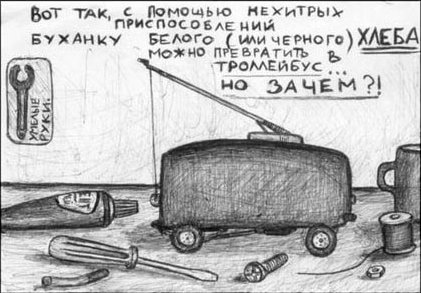
\includegraphics[width=\textwidth]{logo/trolley.jpg}

\bigskip
Редакция: $<$\href{mailto:dponyatov@gmail.com}{dponyatov@gmail.com}$>$

\bigskip
\href{https://github.com/ponyatov/scratcher}{
\includegraphics[height=5em]{logo/GitHub.png}}
\ 
\includegraphics[height=3em]{logo/linuxpowered.png}
\ 
\includegraphics[height=5em]{logo/OpenHardware.png}
{\Large Powered by \LaTeX}

\end{titlepage}

\tableofcontents\clearpage

\section{Об этом журнале\\Сделай сам, расскажи другим}
\begin{multicols}{2}

Наблюдая современные информационные тренды в \internet е, можно заметить, что
большое внимание уделяется различным самоделкам, DIY, 3D-принтерам, любительской
электронике и концептам различных гаджетов.

Если попробовать взглянуть немного дальше, можно заметить все более и более
заметное развитие такого явления как <<Персональное производство>>\ --- большой
интерес вызывает возможность создания и изготовления уникальных вещей, 
нужных только конкретному человеку.

С другой сторны, все усложняющиеся вещи и технологии вызывают у людей желание
начать с нуля, создать что-то пользуясь старыми приемами. В клинических
случаях попадаются особи, испытывающие дикий баттхерт от глобализации и
массового производства, и бегущие подальше от цивилизации, прихватив с собой
генератор и мобильник с \internet ом \smiley.

\emph{
Вполне можно ожидать, что эти тенденции приведут к появлению и оформлению нового
культурного течения, которое можно назвать} \textbf{скрэтчинг}\footnote{\ тут бы
хорошо подошло слово <<рукоблудие>>, но термин к сожалению уже занят, а
другого русского аналога подобрать пока не удалось}.

Этот журнал создан для \scr ов\ --- людей, чье хобби создавать вещи и технологии
по следам уже существующих, в сотый раз изобретать велосипед, чтобы разобраться
как оно работает, научиться делать самому, а возможно найти новый или забытый
способ что-то сделать, и конечно получить удовольствие от процесса поиска. 

\end{multicols}

\section{КопиПаста\\Как сказать "Начать с нуля"\ ?}
\begin{multicols}{2}

\begin{itemize}
  \item
На английском — to start from scratch; to start over.
  \item
На испанском — empezar de cero; empezar de nuevo.
  \item
На итальянском — partire dal niente.
\end{itemize}

В общем-то во всех языках мы видим <<кальку>>, выделяется только одно,
содержащее слово <<scratch>> (царапина, черта).

С момента его возникновения, это выражение немного поменяло свое значение.
Сейчас оно используется, когда мы хотим сказать <<начать снова, начать с
начала>> в том смысле, что мы потерпели поражение при первой попытке.

Фраза родилась в конце 19-го века и тогда просто значила <<начинать без
преимуществ>>. Слово <<scratch>> использовалось с 18-го века как спортивный
термин, обозначающий линию старта, прочерченную на земле. Впервые такая линия
упоминалась в описании игры в крикет\ --- на ней стоял игрок, отбивающий мяч.

<<Start from scratch>> в качестве понятия <<начинать с нуля>> пришло к нам из
бокса. Прочерченная линия определяла позиции боксеров, когда они стояли друг
напротив друга в начале поединка. Отсюда также произошло выражение <<up to
scratch>>, (быть на должной высоте, в прекрасной форме), т.е. соответствовать
стандартам, предъявляемым боксерам, делающим заявку на матч.

Позднее <<scratch>> стали называть любую стартовую точку в бегах. Термин стали
использовать в <<гандикап>>-соревнованиях (handicap), в которых более слабый
участник получает фору. Например, в велоспорте те, у кого нет преимуществ, стоят
на линии, в то время как остальные стоят впереди. Другие виды спорта, особенно
гольф, заимствовали переносное значение <<scratch>> как термин для обозначения
<<без преимуществ\ --- начинать с нуля>>.

В The Fort Wayne Gazette (апрель 1887) содержится самое раннее упоминание <<start
from scratch>> — в репортаже о <<‘no-handicap>> велосипедной гонке:

<<It was no handicap. Every man was qualified to and did start from scratch.>>

По моим наблюдениям, <<start from scratch>> употребляется чаще в письменной речи
(например, уже несколько раз видела его в статьях в интернете), а <<to start
over>>\ --- в разговорной (слышала в американском сериале).

\bigskip
\copyright\ \href{http://www.lingvaroom.ru/kak-skazat-nachat-s-nulya/}{Юлия
Горбунова}

\end{multicols}

\section{КопиПаста\\Персональное производство\\еще один шаг к реконизму}
\begin{multicols}{2}

Один из важных моментов в построении реконистической экономики — это
трансформация традиционного, корпоративного производства, основанного на
обязательной организации, как в смысле объединения людей, средств производства,
финансовых и материальных ресурсов, так и в смысле появления так называемых
юридических лиц как практически единственных субъектов производства. Такое
производство в значительной части сфер деятельности будет вытесняться
индивидуальным производством, когда  любой желающий, используя так называемые
микрофабрики — миниатюрный комплект универсального оборудования, сможет
производить достаточно широкую линейку продукции, как для личного пользования,
так и для продажи. Произойдет нечто вроде возврата к ремесленному производству
средневековья и даже к натуральному хозяйству, но на неизмеримо более высоком
технологическом уровне. Особую ценность в таких условиях обретет информация —
продаваться будет не товар, а инструкция для микрофабрики, как данный товар
изготовить. Конечно, такие инструкции будет не только продаваться, но и
распространяться бесплатно, а также вороваться. Разумеется, это серьезно
поменяет привычную нам социально-экономическую систему.

В последнем номере журнала «Наука и жизнь» (№8 за 2012 год), появилась небольшая
заметка, в которой рассказывается о разработке профессора Массачусетского
технологического института Нила Гершенфельда, который предложил концепцию
миниатюрной фабрики-лаборатории (Fab Lab). Фабрика-лаборатория представляет
собой комплекс станков, совместно работающих под управлением персонального
компьютера. Идея Гершенфельда получила широкое распространение и десятки
университетов и исследовательских центров экспериментируют с такими
мини-фабриками. В России первая такая фабрика создана в Московском институте
стали сплавов, в ее составе фрезерный станок для обработки древесины, пластиков
и мягких металлов, гравировальный прецизионный станок для производства печатных
плат, установка лазерной резки, плоттер для раскроя гибких материалов и
производства гибких микросхем, и 3D-принтер, предназначенный для изготовления
любых изделий из ABS-пластика.

Так что, возможно, что лет через десять, для того чтобы поменять надоевший
мобильный телефон, мы будем заходить на сайт какой-нибудь Нокии, скачивать файл
с данными, запускать его в программе на домашнем компьютере, а стоящий на
тумбочке агрегат, очертаниями смахивающий на современное МФУ, погудев пару
минут, выбросит в приемный лоток еще горячую, пахнущую свежим пластиком
мобилку\ldots
\smiley

\bigskip
\copyright\
\href{http://blog42.ws/personalnoe-proizvodstvo-eshhe-odin-shag-k-rekonizmu/}{AG}

\end{multicols}

\section{Новости технологий\\Злобный янки в
3D-танке\\Полевые 3D-принтеры на службе американской армии}
\begin{multicols}{2}

Пока специалисты в области 3D-печати рассуждают о перспективах приенения
технологии, а энтузиасты осторожно говорят о потенциальной возможности печати
необходимого скарба сразу на лунной базе (чтобы не тащить лишнее с Земли),
американская армия без всяких промедлений нашла применение 3D-печати уже сейчас.
Военные США стали использовать мобильные лаборатории Expeditionary Lab Mobile с
3D-принтерами в комплекте.

\end{multicols}
\noindent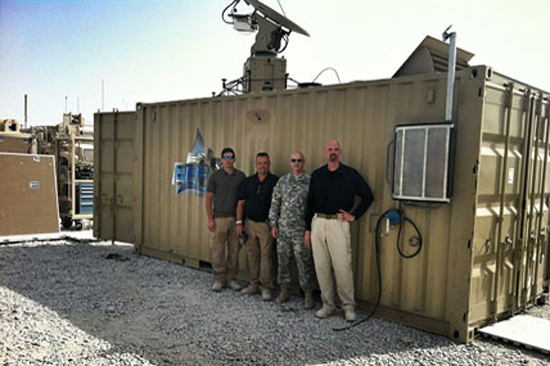
\includegraphics[width=\textwidth]{fig/00/01.jpg}

\noindent\textbf{Чебураторы на тропе войны}
\begin{multicols}{2}

Основными задачами лабораторий Expeditionary Lab Mobile (сокращённо — ELM) будет
изготовление одноразовых инструментов для нужд армии, а также внесение
корректирующих дополнений в уже существующее оборудование — «полевое»
использование часто требует определённой доводки. В качестве примера приводится
случай, когда войска получают партию карманных фонарей с дефектом – быстро
выходящим из строя предохранителем выключателя. Находясь в кармане у военного,
такой фонарь может самопроизвольно включиться и либо выдать местонахождение
бойца, либо впустую разрядить батарейки. Однако, имея под рукой ELM, можно
быстро допечатать предохранители, без необходимости отсылки всей партии обратно
в США для замены. 

% \end{multicols}
\noindent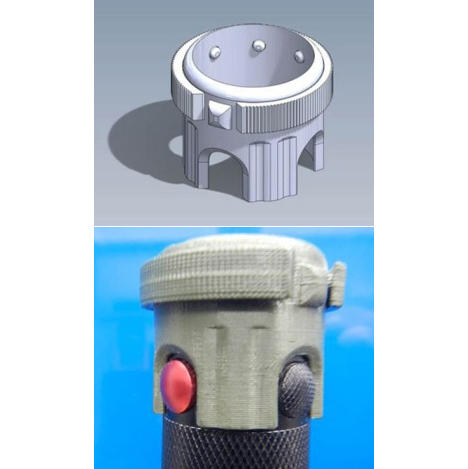
\includegraphics[height=0.5\textheight]{fig/00/03.jpg}
% \begin{multicols}{2}

Ещё одним примером можно назвать реальный случай недоработки в
конструкции миноискателя, приведший к тому, что время работы прибора из-за
иракской жары сократилось с восьми часов до 45 минут. В результате во время
многодневных миссий солдаты были вынуждены носить большое количество
дополнительных батарей. Использование ELM позволило сконструировать адаптер для
использования батарей другого типа и увеличить время работы миноискателя до
девяти часов.

Expeditionary Lab Mobile представляет собой стандартный грузовой контейнер
(6,1$\times$2,4 м), внутри которого находятся 3D-принтер, специальные станки с
ЧПУ (для изготовления более сложных деталей из стали и алюминия) и набор
традиционных инструментов: резак, сварочный аппарат, циркулярная пила,
маршрутизатор, лобзик и сабельная пила. Кроме того, в комплекте ELM имеется
спутниковое оборудование связи для проведения телеконференций с чиновниками и
инженерами в США – для оперативных корректировок работы. При каждой лаборатории
будут находиться два инженера. Все лаборатории будут связаны между собой единой
компьютерной сетью.

% \end{multicols}
\noindent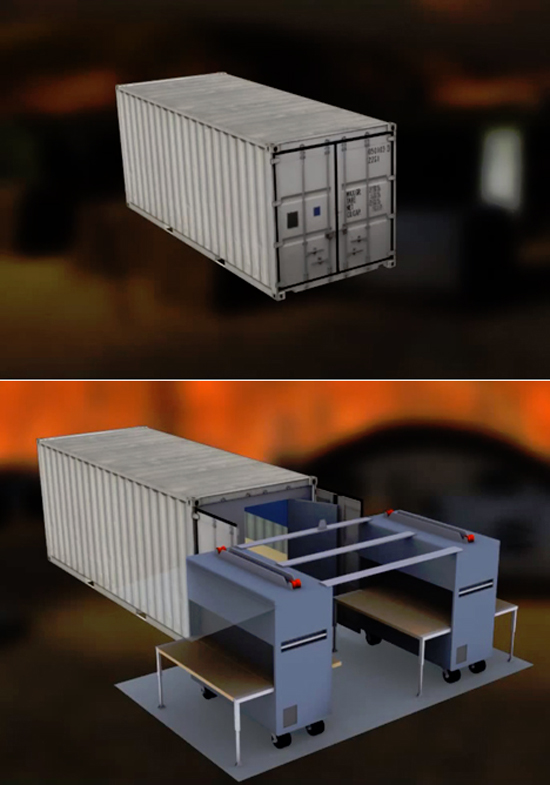
\includegraphics[width=\columnwidth]{fig/00/02.jpg}
% \begin{multicols}{2}

Стоит отметить, что подобный способ изготовления износившихся или недостающих
деталей довольно дорог: стоимость каждой лаборатории составляет около 2,8
миллиона долларов. Планируется, что первые ELM будут испытаны в Афганистане.
Кроме того, можно надеяться, что успешное применение новых технологий на <<поле
боя>> будет способствовать их внедрению для мирных операций. Например, во время
стихийных бедствий.

\bigskip
\copyright\
\href{http://www.computerra.ru/50860/polevyie-3d-printeryi-na-sluzhbe-amerikans/}{Компьютерра, Николай Маслухин}

\end{multicols}

\section{Принципы скрэтчера\\Чем оно отличается от прочего DIY}
\begin{multicols}{2}

\begin{itemize}
  
\item Из говна и палок
  
Чем больше г и кривее палки, тем круче \scr
  
\item Сделай сам, расскажи другим
  
Необходим активный обмен информацией для мимимизации и так больших расходов на
избретение колес
  
\item Минимум покупных изделий

В идеале изготовление всего из чисто природных материлов и без стартового
инструмента

\item Все покупные ништяки должны быть всегда доступны в любом ближайшем
магазине

Чтобы каждый мог легко и быстро повторить понравившийся хак.

\emph{Следует обратить внимание, что этому принципу противоречит использование
техно-мусора, различных деталей от старой техники и т.п.\ --- вот сколько
сейчас у вас например сломанных стиралок, или дохлых телевизоров в доме ?}

\emph{Еще одно противоречие\ --- покупка комплектухи по почте в Китае, и заказ
редких компонентов в магазинах}

\item Покупаться должны \textbf{самые дешевые}\ и самые кривые
комплектующие

Но при этом не нужно скатываться на использование раритета\ --- см. доступность.

\item Приоритетно использование более ранней ступени
\term{технологического передела}

Например вместо использование готового заводского сверла взять хвостовик от
сломанного, и выпилить сверло самому. Правильнее было бы взять твердосплавную
заготовку, но это противоречит принципу доступности, т.к. их нет в
доступных магазинах. Вариант использование куска проката из инструментального
сплава лучше, потому что можно еще повыделываться с термичкой \smiley

\item Должно использоваться \term{открытое программное обеспечение}

Причем написанное целиком самостоятельно на ассемблере, ну или хотя бы собрать
\href{http://cross-lfs.org/}{Cross Linux From Scratch}\ для DIY компьютера,
спаянного из отдельных деталей с помощью самодельного паяльника.

В процессе неплохо попутно изобрести пару уникальных языков программирования,
написать на них операционную систему и комплект программного обеспечения.

\item Желательно использовать нетиповые приемы работы и технологии

\item При разработке конструкций нужно стремиться использовать малоизвестные и
уникальные конструктивные решения

\item Максимум самодельного инструмента

\item Идеал \scr а\ --- пройти всю технологическую цепочку от каменного 
рубила до обрабатывающего центра с ЧПУ

И с разгона заскочить еще дальше, обогнав текущие лабораторные разработки по
3D-печати, зональной плавке и прочим свежакам технологии

\item Минимум повторов готовых изделий и унификации

Каждая поделка должна быть прекрасна в своей уникальности, и ее область
применения должна быть максимально узкозаточенной под ваши задачи. Применение
унификации, общеизвестных конструктивных решений и принципов работы неприемлемо,
т.к. какой смысл повторять уже готовое изделие, которое можно купить ?!

\item Больше науки

Копайте книги по математике, физике и химии, больше статей и техрасчетов.
Чем больше матана и самопала, тем выше левел. Не забывайте про пропагандизм
достижений на форумах (особенно нетематических) и в оффлайне.

\item Больше синей изоленты

\item Обязательно используйте ардуину

Даже если устройство вообще не предполагает использование электричества\ ---
прикрутите микроконтроллер изолентой, и подключите к нему компьютер.

\item Для успеха проекта обязательно нужен ковер

\item На демонстрационном видео должно что-нибудь отвалиться или чпохнуть
волшебным синим дымом
   
\end{itemize}	

\end{multicols}

Набор принципов \scr а выглядит похоже на инструкцию <<Как просрать полимеры>>,
поэтому как и в любом другом деле, не нужно доводить их исполнение до фанатизма.
\emph{Новизна и уникальность} на первом месте, и не надо забывать что это все же
хобби, а не жизненная миссия. Нужно всего лишь следить за соблюдением баланса
между потраченными средствами, временем, и полученным от процесса удовольствием.

Главное достоинство отработанных вещей и технологий\ --- на их доводку и
проверку уже было потрачено гигантское количество ресурсов. Самодельные аналоги
в любом случае будут хуже и на порядок дороже, чем серийное изделие, за редким
исключением узконишевого использования, для которого готовое решение почему-то
не подходит.

Из положительных эффектов \scr ства можно отметить хорошие общетехнические
знания, и умение при необходимости быстро слепить <<костыль>> (временное решение
проблемы) из подручных ресурсов.

\section{Инструмент\\Кустарь-одиночка с мотором}
\begin{multicols}{2}

\href{https://www.youtube.com/playlist?list=PL6mXlWgvuzAu4jMVzOOKXXDVF3r1yAaz4}{Отличная
серия видео по изготовлению токарника}

Возникает вопрос, где взять самый дешевый, легко доставаемый и универсальный
электропривод, и нужно ли вообще пользоватся электричеством.

Вопрос по использованию электричества оставляем самым упоротым \scr ам 80-го
левела. Будем исходить из того, что хоть какое-то (под нагрузку мощностью от
100$\div$200\,Вт) сетевое электричество доступно сейчас всем, кроме туристов,
огородников и прочих полевиков, не укомплектованных бензогенератором.

\emph{Соответственно в комплекте базового инструмента предполагаем наличие
минимум электродрели и паяльника.}

\noindent\href{http://leroymerlin.ru/catalogue/instrumenty/elektroinstrument/dreli\_udarnye/13805983/}{
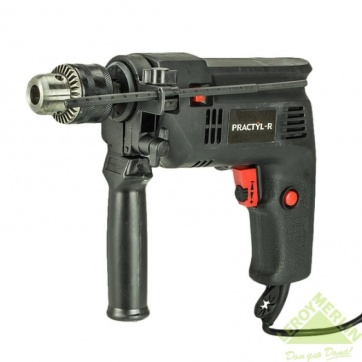
\includegraphics[width=\columnwidth]{fig/00/PraktylR.jpg}}
\textbf{Дрель ударная сетевая Praktyl-R 400 Вт (!)395\,р.}

\noindent\href{http://leroymerlin.ru/catalogue/instrumenty/elektroinstrument/dreli\_bezudarnye/11857763/}{
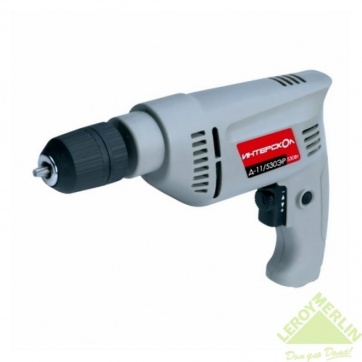
\includegraphics[width=\columnwidth]{fig/00/D_11_530ER.jpg}}
\textbf{Дрель безударная сетевая Интерскол Д-11/530ЭР (с БЗП) 1120\,р.}

Дрель\ --- голимая китайчатина от 400\,р, по надежности рекомедуется Интерскол
1100+\,р. Надежность Интерскола\ --- не <<китай>>, классика ДУ-580ЭР
работает в хвост и гриву в университете ежедневно с $\sim$2005 г., используется
криворукими студентами, лежит в подвале в пыли от точила, и никаких вопросов
даже со щетками.

Если не планируете много сверлить бетон, \textbf{берите дрель без ударного
механизма}: отсутствуют лишние продольные перемещения, что может быть важно при
использовании в качестве шпинделя сверлильного станка, и механизации других
технологических поделок.

\emph{Шуруповерт\ --- буржуйство, у него нет 43\,мм шейки для фиксации, поэтому
как средство электропривода он практически бесполезен, и нужен собственно для
заворачивания большого количества саморезов. Хотя наличие ограничителя
крутящего момента и малые габариты удобны при сверлении и сборке поделок.}

\noindent\href{http://leroymerlin.ru/catalogue/instrumenty/elektroinstrument/lobziki/13805991/}{
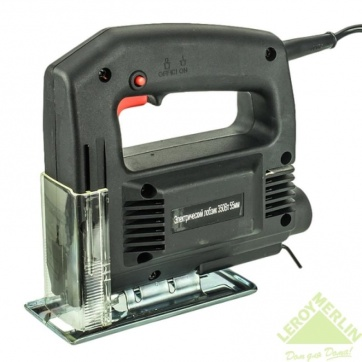
\includegraphics[width=\columnwidth]{fig/00/LobzPraktyl.jpg}}
\textbf{Лобзик Praktyl 350 Вт 356\,р.}

\noindent\href{http://leroymerlin.ru/catalogue/instrumenty/elektroinstrument/lobziki/12114283/}{
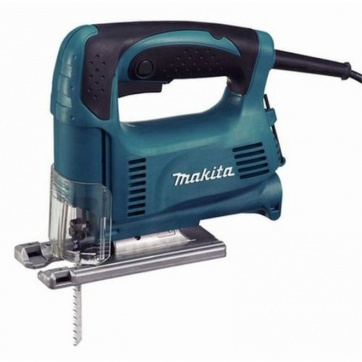
\includegraphics[width=\columnwidth]{fig/00/LobzMakita4329.jpg}}
\textbf{Лобзик Makite 4329 2260\,р.}

Лобзик опционален, и куда полезнее шуруповерта, китай-хлам 
350+\,р, чуть поприличнее 2000+\,р. 
\textbf{Не берите с маятником дешевле 5--7\,тыс.р}.

\noindent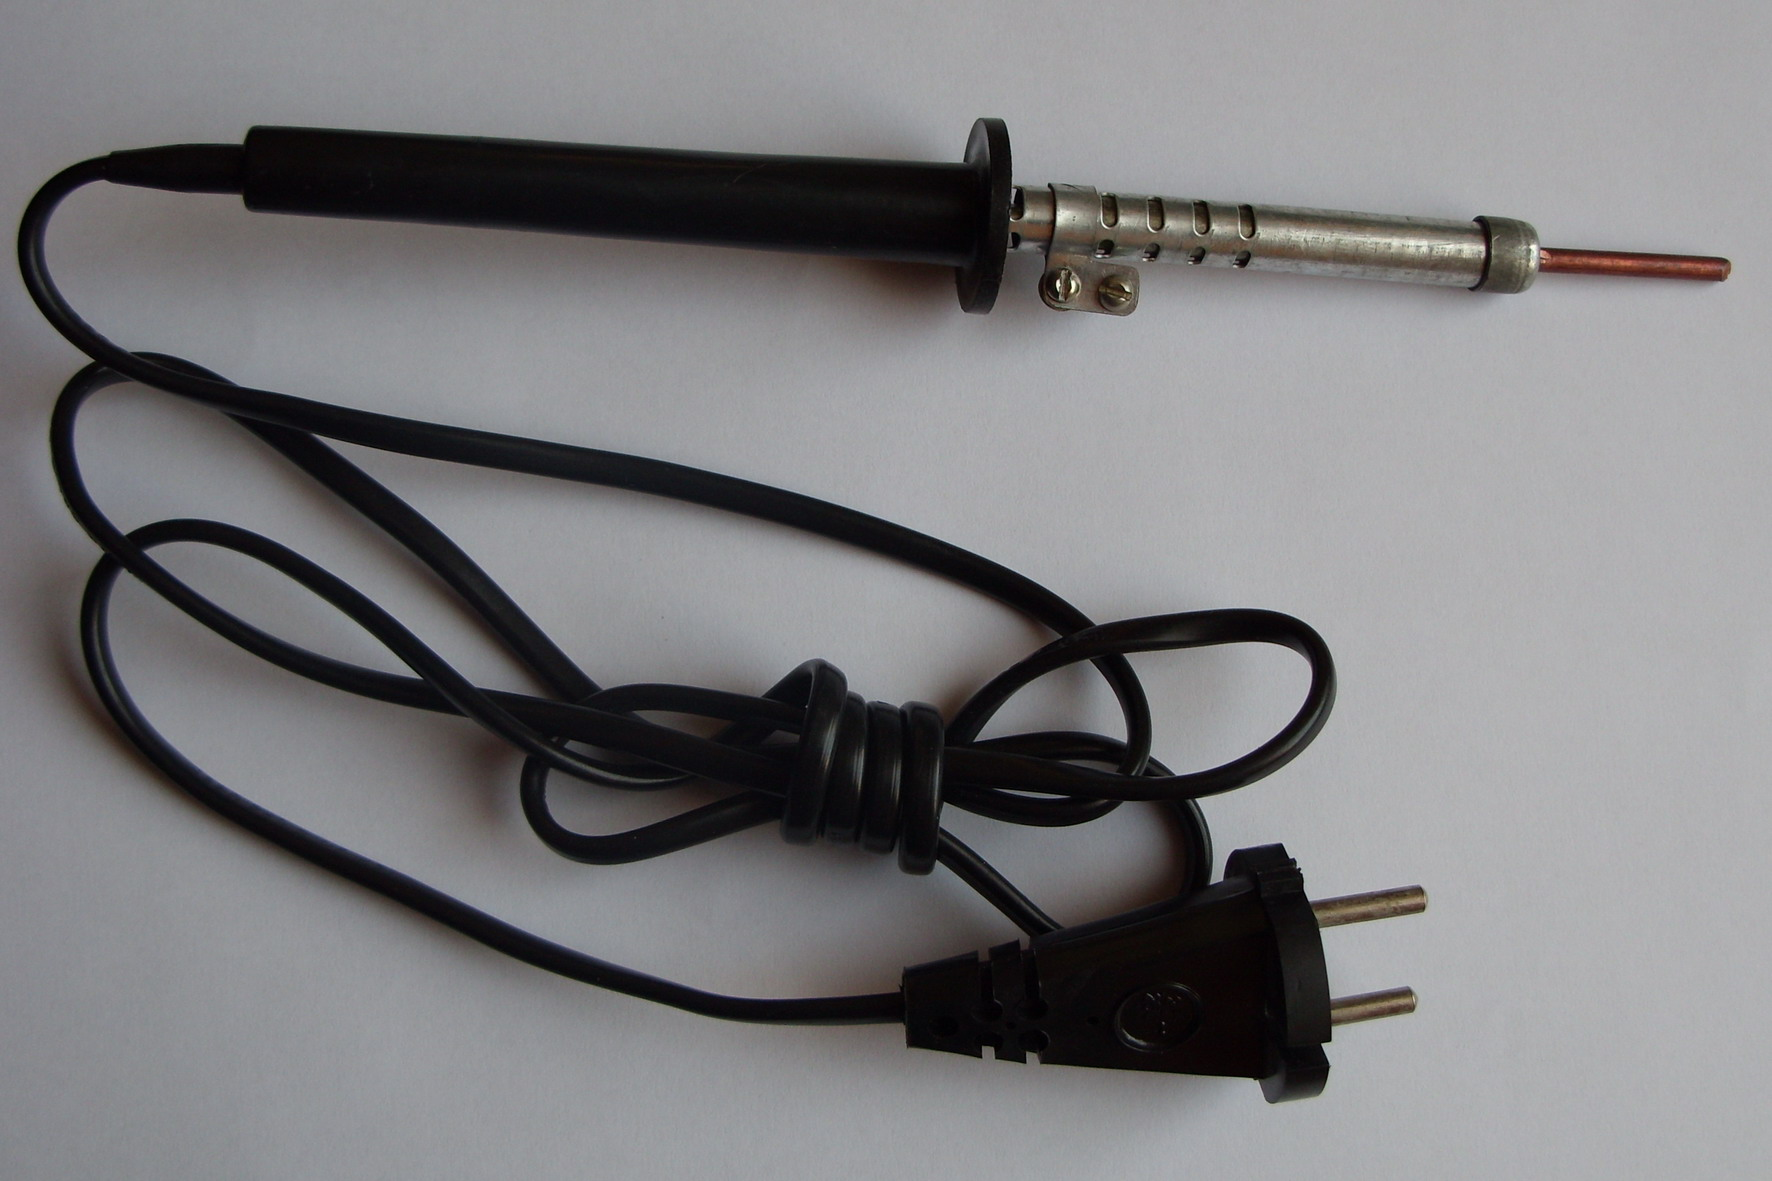
\includegraphics[width=\columnwidth]{fig/00/EPSN25.jpg}
\textbf{Паяльник ЭПСН-25/220}

\noindent\href{http://voltmaster-samara.ru/catalog/product/00067650/}{
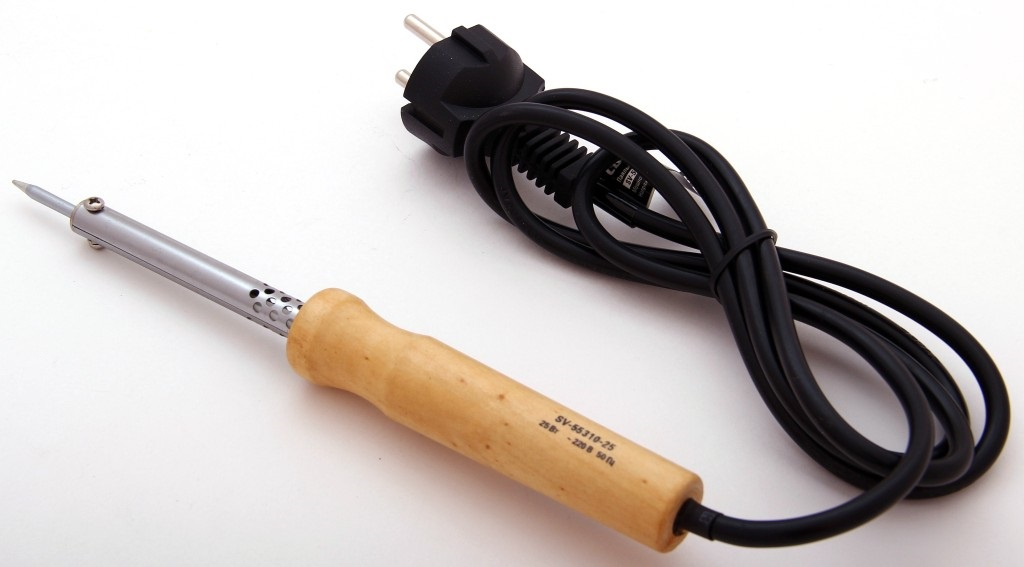
\includegraphics[width=\columnwidth]{fig/00/SV-55310-25.jpg}}
\textbf{Паяльник 220В 25Вт, СВЕТОЗАР, SV-55310-25 230\,р.}

\noindent\href{http://voltmaster-samara.ru/catalog/product/00091478/}{
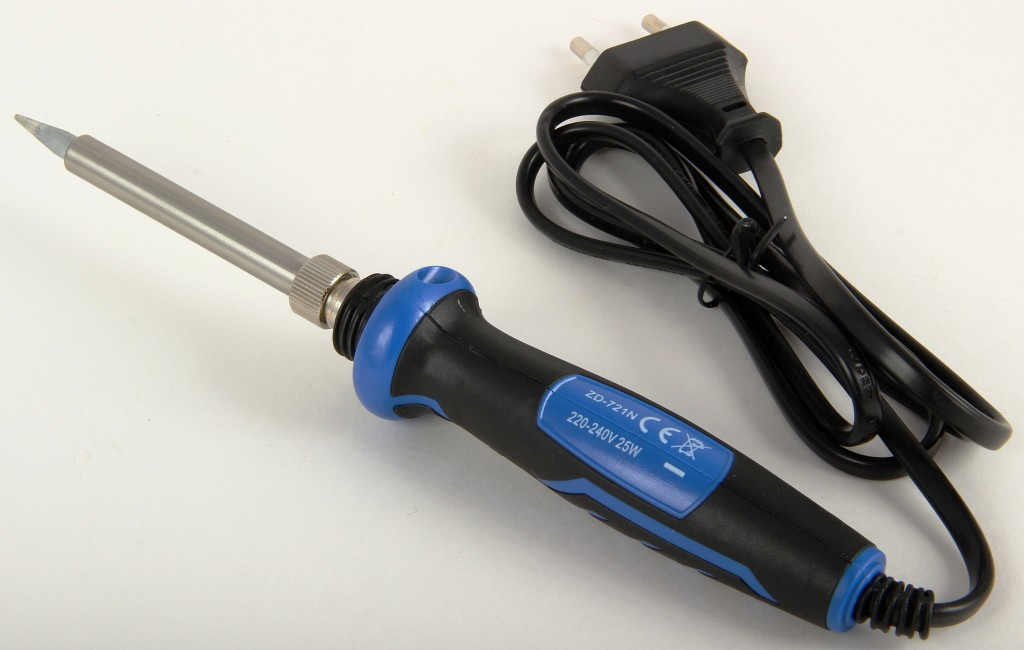
\includegraphics[width=\columnwidth]{fig/00/ZD-721N.jpg}}
\textbf{Паяльник 220В 25Вт ZD-721N 175\,р.}

Паяльник\ --- обязателен дешевый сетевой мощностью не менее 20\,Вт, типа
ЭПСН-25/220.
\emph{Ограничитель мощности или регулятор температуры труъ-\scr\ должен собрать
самостоятельно.}

\noindent\href{http://voltmaster-samara.ru/catalog/product/00047380/}{
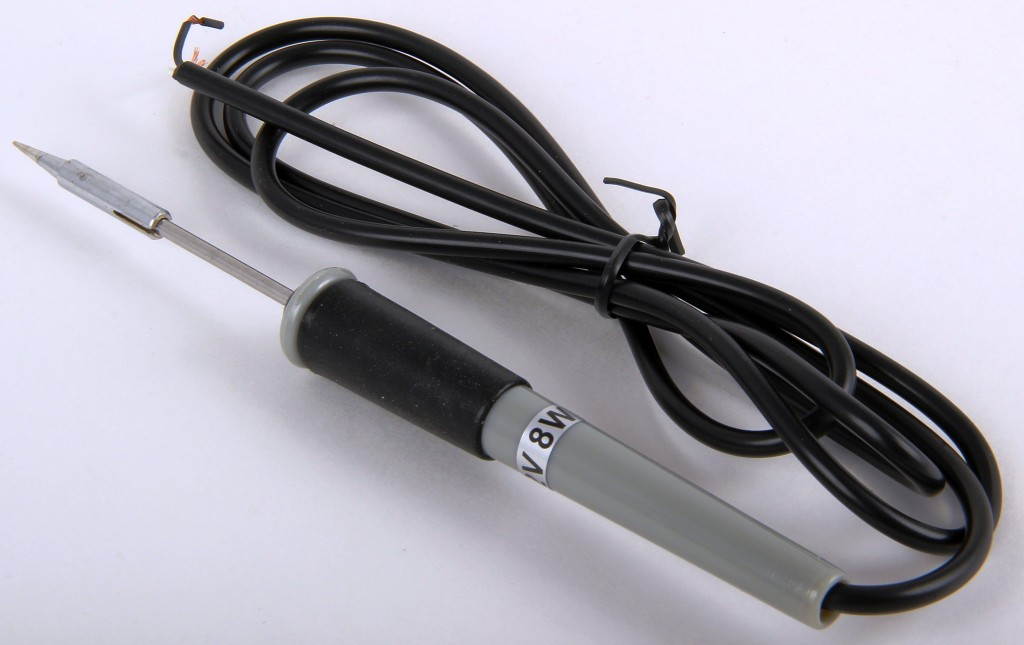
\includegraphics[width=\columnwidth]{fig/00/Iron8W.jpg}}
\textbf{Паяльник для станции ZD-927 12\,В 8\,Вт 85\,р.}

Для сборки электроники хорошо также иметь маленький монтажный 12\,В 8\,Вт от
паяльной станции ZD-927 ($\sim$100\,р), без самой станции. 

\noindent\href{http://voltmaster-samara.ru/catalog/product/00073790/}{
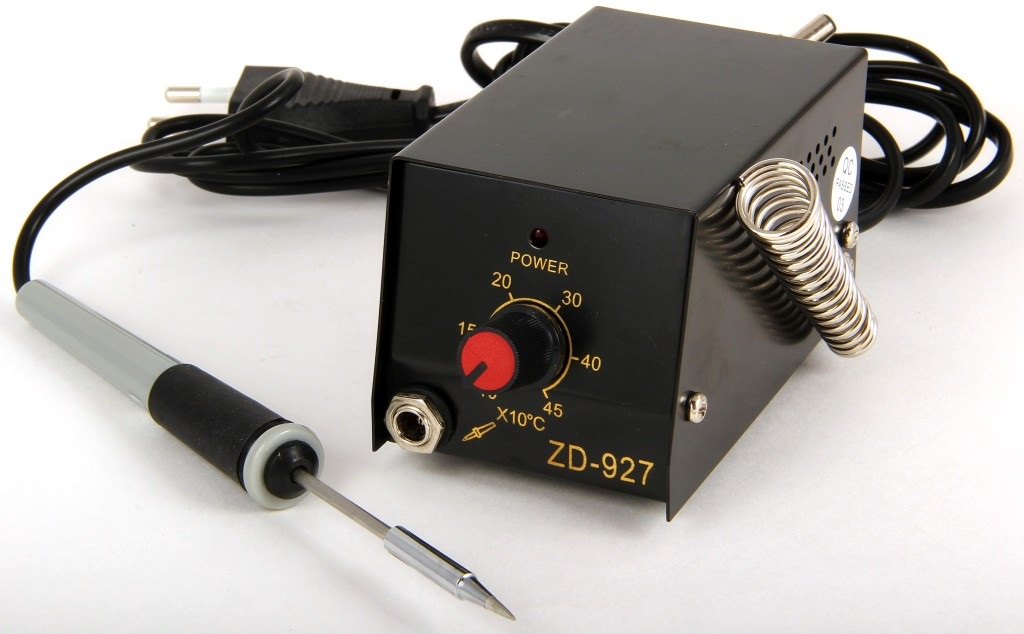
\includegraphics[width=\columnwidth]{fig/00/ZD927.jpg}}
\textbf{Паяльная станция ZD-927 520\,р.}

Если не жалко 500\,р, берите ZD-927 целиком, внутри простейший регулятор
мощности, и вам не понадобится источник питания на 12\,В, который вы еще не
сделали. \emph{Но труъ путь\ --- конечно собрать свой паяльник целиком, из
нихрома, жала из толстой проволоки или медной шины, и самостоятельно выточенной
ручки.}

\noindent\href{http://voltmaster-samara.ru/catalog/product/00073444/}{
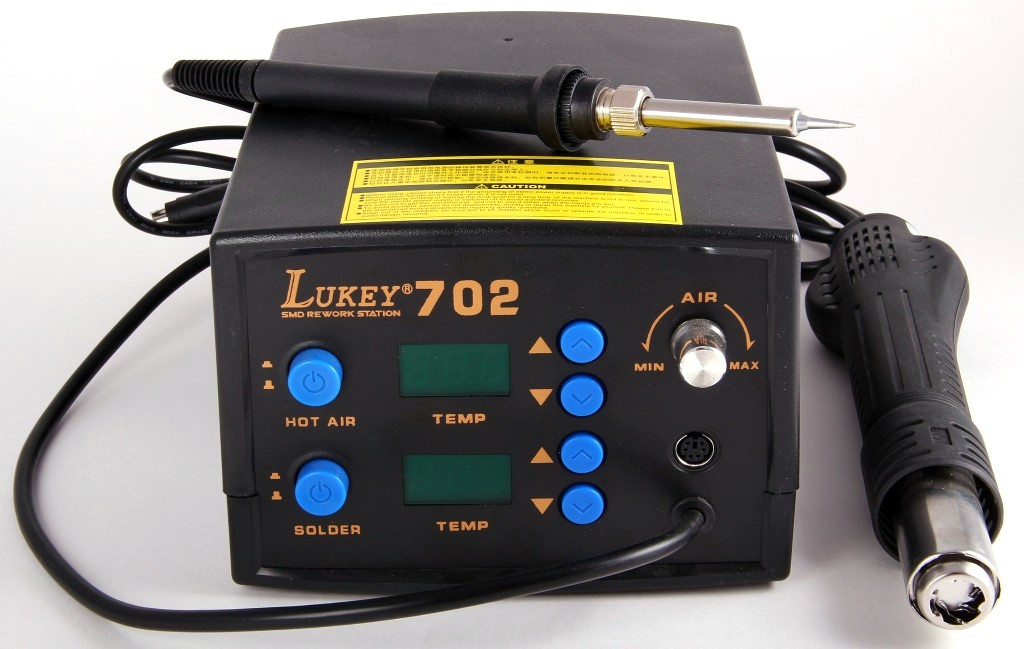
\includegraphics[width=\columnwidth]{fig/00/Lukey702.jpg}}
\textbf{Паяльная станция LUKEY 702 3100\,р.}

\noindent\href{http://shop.siriust.ru/product\_info.php/cPath/23\_28\_269/products\_id/15290}{
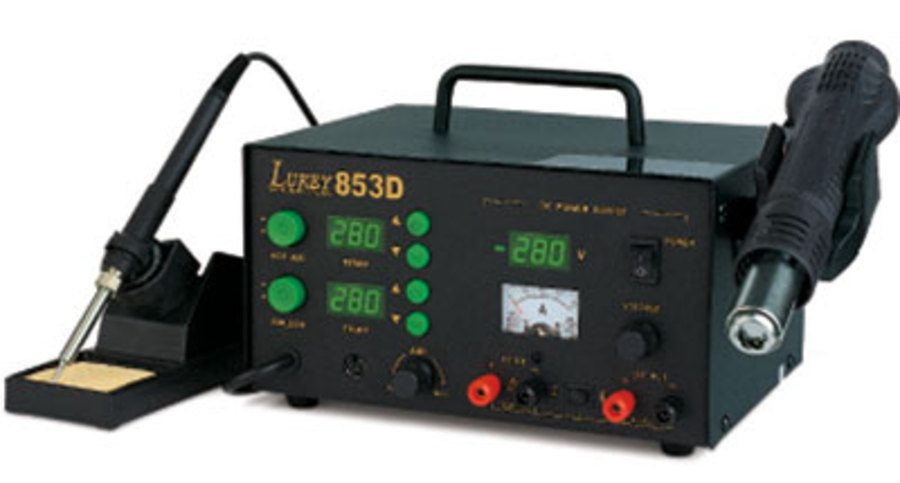
\includegraphics[width=\columnwidth]{fig/00/Lukey853D.jpg}}
\textbf{Паяльная станция LUKEY 853D с простым источником питания 5200\,р.}

Паяльные станции типа Lukey 702/853D (3000+\,р) естественно не рассматриваем
\smiley. Для работы или регулярного хобби паяльная станция с феном, а может даже
и встроенным источником питания, вещь незаменимая, и не такая уж дорогая, но для
\scr а слишком технологичная.

\bigskip

Первый кандидат на место универсального электропривода достается той
самой дрели, не забываем об обязательном наличии 43\,мм монтажной шейки.
Достоинство дрели как привода\ --- прямое подключение к сети, встроенный
редуктор, есть модели с простой регулировкой оборотов, резьба и отверстие под
винт на валу, в комплекте есть патрон для зажима мелких деталей в
точилке\footnote{\ БЗП удобен, патрон с ключем дает лучший зажим и возможно
точнее}

\noindent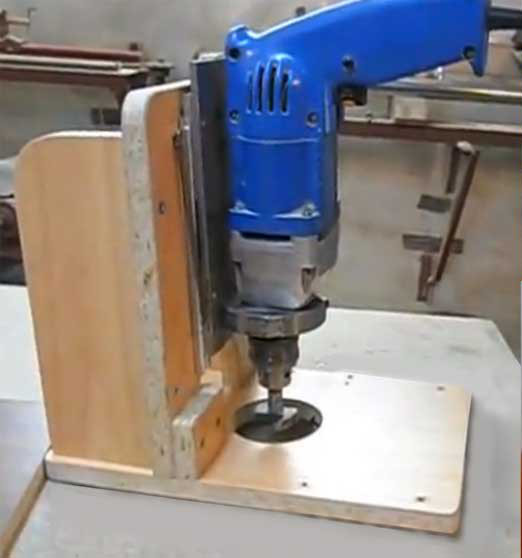
\includegraphics[width=\columnwidth]{fig/00/DrelBoren.jpg}

\noindent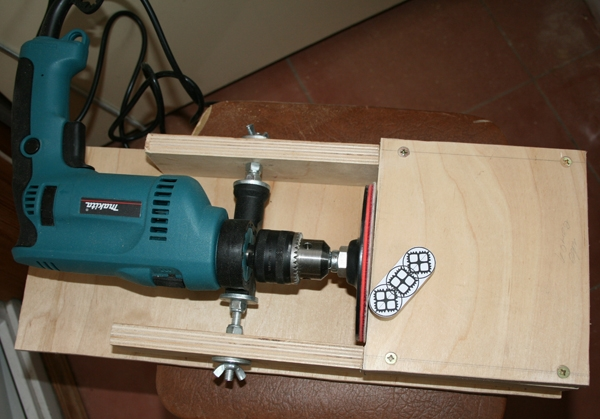
\includegraphics[width=\columnwidth]{fig/00/DrelShliph.jpg}

\noindent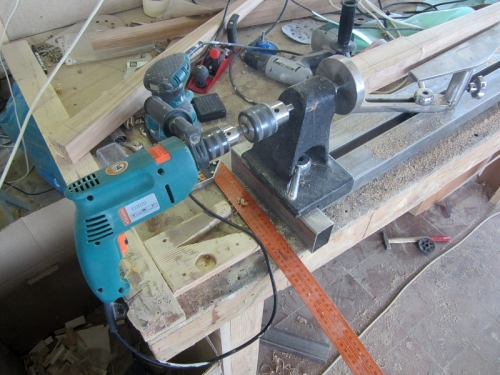
\includegraphics[width=\columnwidth]{fig/00/DrelLathe.jpg}

\noindent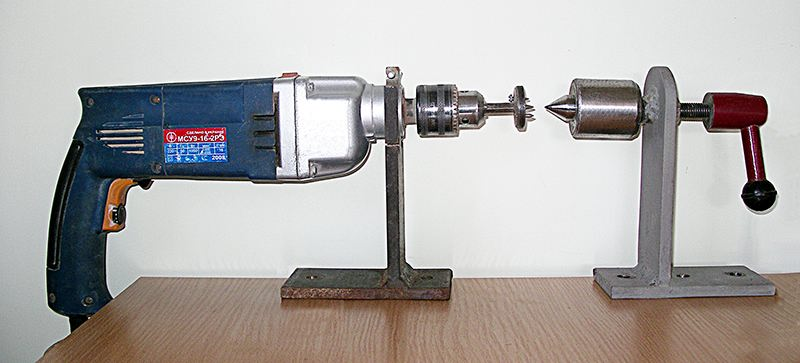
\includegraphics[width=\columnwidth]{fig/00/DrelLathe2.jpg}

\bigskip
Ограниченно доставаемые двигатели от стиральных машин, отличаются
  мощностю и оборотистстью, особенно от старых моделей
  
\noindent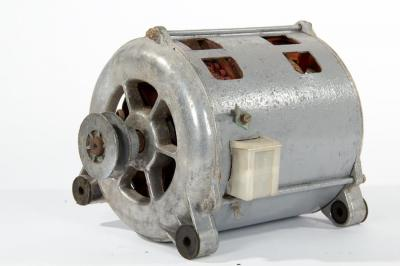
\includegraphics[width=\columnwidth]{fig/00/VyatkaDvig.jpg}
\textbf{Жвигатель Вятка-Автомат 19??\,г.}
  
\bigskip
Автозапчасти: привод печки Камаза, двигатель постоянного тока 24\,В
  50\,Вт
  
\noindent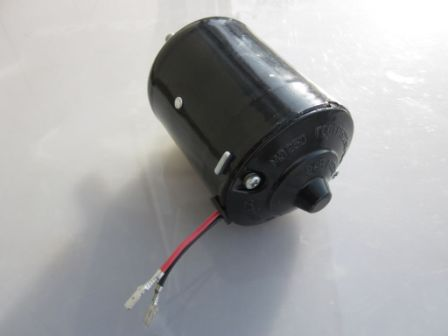
\includegraphics[width=\columnwidth]{fig/00/KamazDvig.jpg}
  
\bigskip
Новые асинхронные двигатели АИРЕ 56 B2/B4 (3000/1500 об.)
с заводским конденсатором, подключается к сети $\sim$220\,В, цена от 2500\,р.
С ростом размеров и мощности цена резко повышается.
Следует обратить внимание на возможность монтажа на дополнительный фланцевый
подшипниковый щит, (?) с моделями АИРЕ 80.

\noindent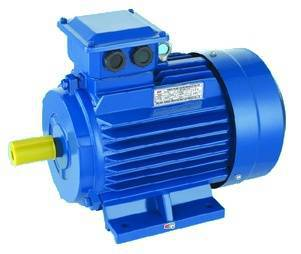
\includegraphics[width=\columnwidth]{fig/00/AIRE.jpg}
\textbf{АИРЕ 56 B2, 0.2\,КВт}

\bigskip
Съемные фрезерные шпиндели, поставляются отдельно или в комплекте с
насадкой ручного фрезера по дереву. Лучшие, со стальной шейкой\ --- Kress,
активно применяются хобби-ЧПУшниками. Попроще и сильно дешевле делал Интерскол,
иногда попадается noname.

Недостаток как универсального привода\ --- они высокоскоростные,
возникают проблемы с понижающими передачами. Применение\ --- приводной
высокоскоростной инструмент: боры, фрезы по дереву, шлифовальные микродиски (?).

\noindent\href{http://kress-shop.ru/product/frezernyj-dvigatel-530-fm-kress-06082302/}{
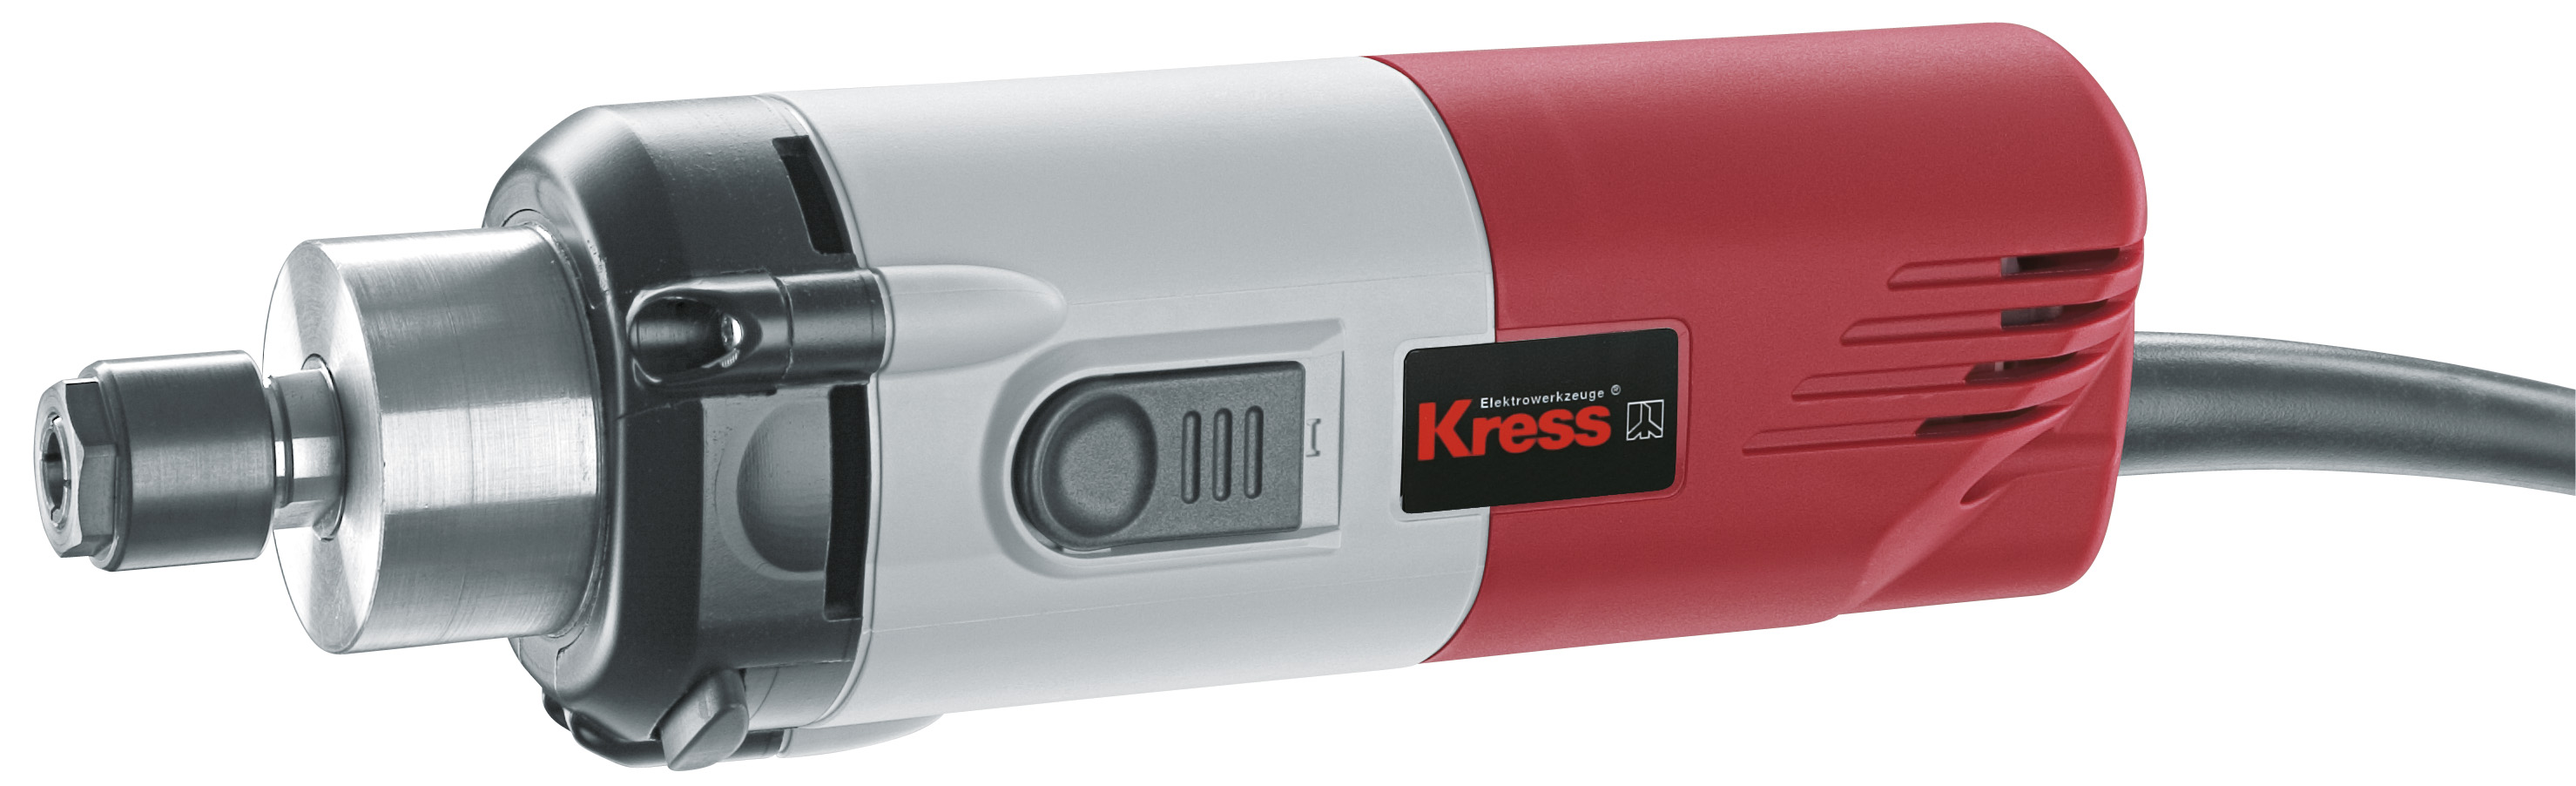
\includegraphics[width=\columnwidth]{fig/00/Kress530.jpg}}
\textbf{Фрезерный двигатель KRESS 530/800/1050 FM(E) 5600+\,р.}

\noindent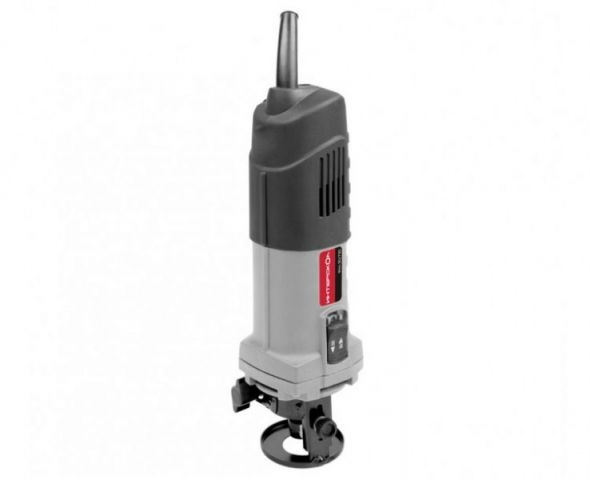
\includegraphics[width=\columnwidth]{fig/00/Interskol30.jpg}
\textbf{Шпиндель Интерскол ФМ-30/750 /снят с производства/}

\noindent\href{http://www.kuvalda.ru/catalog/1867/27920/}{
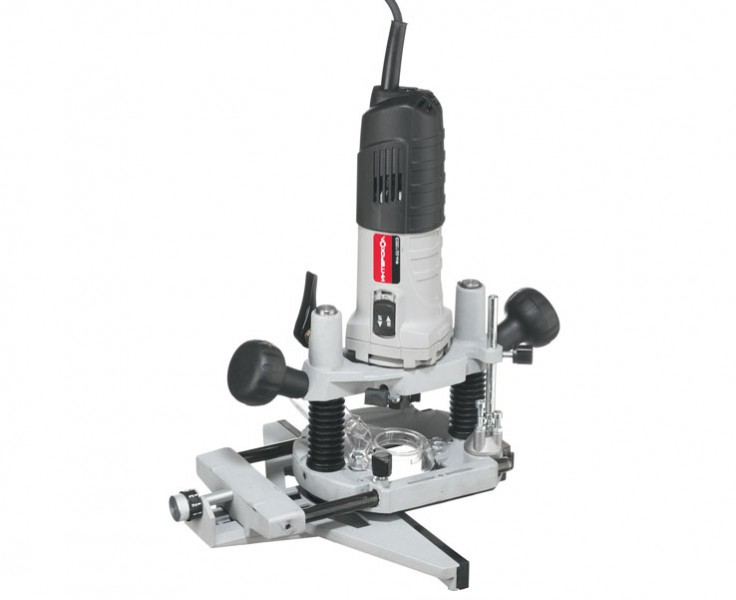
\includegraphics[width=\columnwidth]{fig/00/InterskolFM55.jpg}}
\textbf{Фрезер сетевой Интерскол ФМ-55/1000 Э 5050\,р.}

\bigskip
Китайские воздушные шпиндели постоянного тока с цанговыми патронами ER11:
привод для сверлилки и микроинструмента

\noindent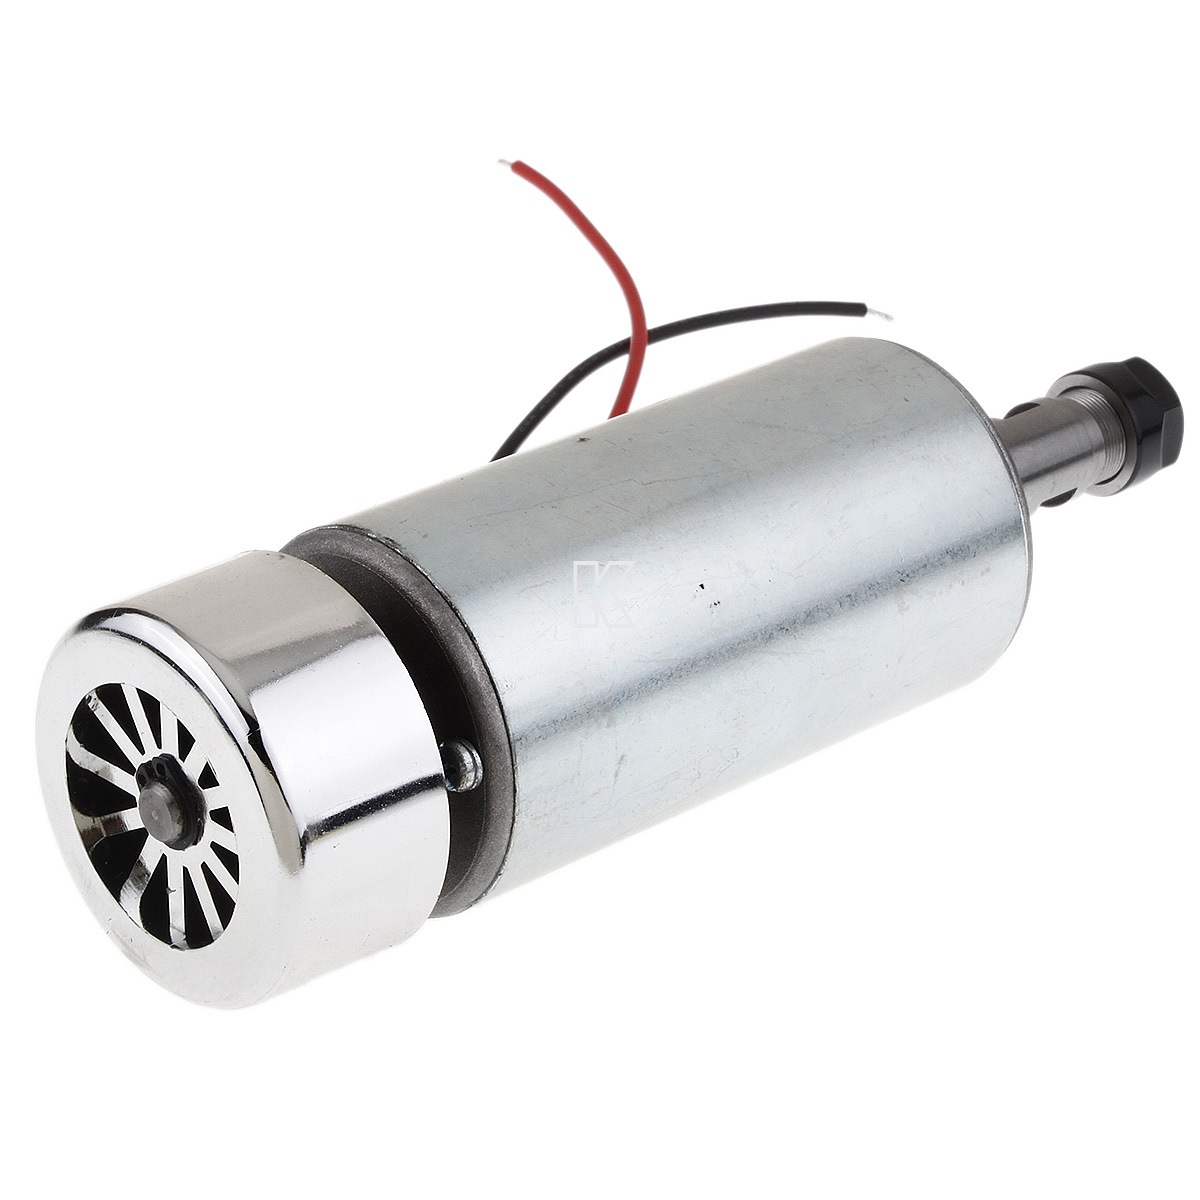
\includegraphics[width=\columnwidth]{fig/00/ER11.jpg}

\bigskip
По мелкому ручному инструменту вопрос открыт.

Учитывая доступность и наличие дешевых вариантов, стоит ли использовать старый
опыт мастеров-ремесленников, когда ученику давали только напильник, и он сам
должен был изготовить себе весь инструмент ?

По крайней мере, вот этот вариант точно не подходит \smiley:

\noindent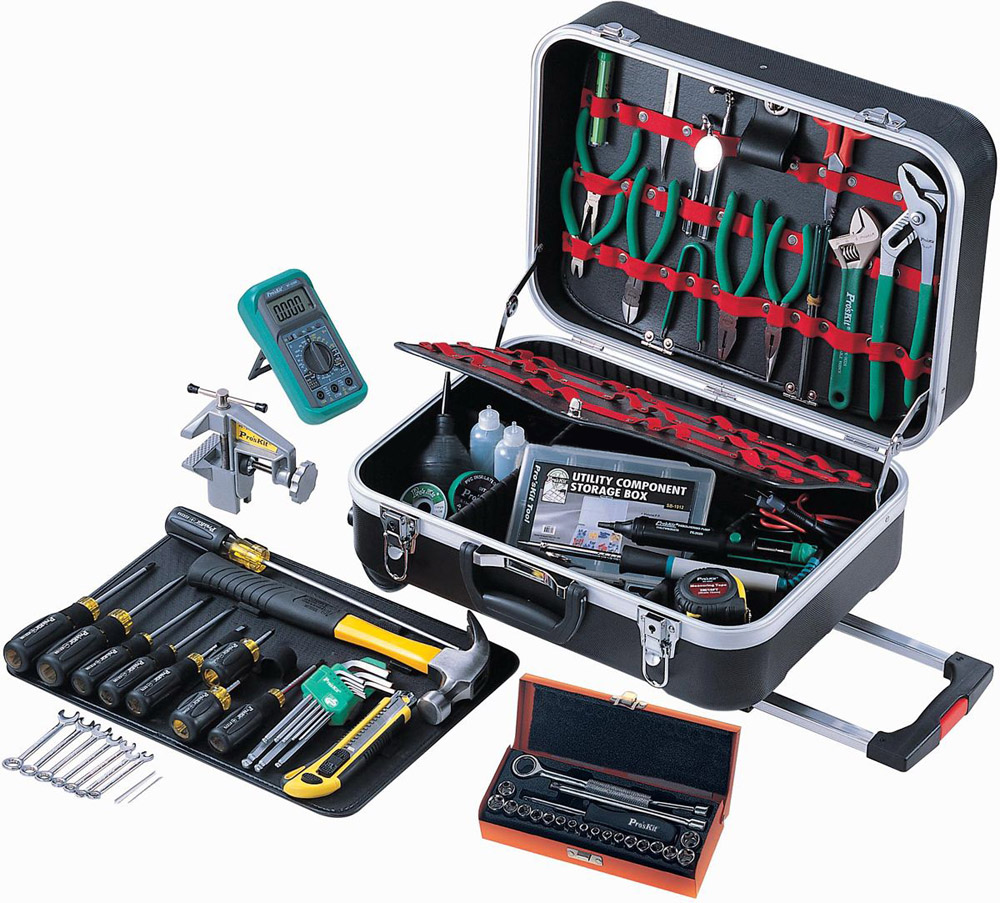
\includegraphics[width=\columnwidth]{fig/00/PK5308BM.jpg}
\textbf{PK-5308BM универсальный набор инструментов ProsKit}

Но пара надфилей, заточной камень на дрель, комплект сверел и несколько листов
наждачки вполне допускаются \smiley.

Если хочется посложнее, можно ограничиться только парой электродвигателей:
\begin{enumerate}
  \item 
относительно медленный высокомоментный АИРЕ 56 B2/4 на силовой привод и
\item 
высокоскоростной 10+ тыс.об$^{-1}$ для сверления, шлифования насадками и т.п.
операции допускающие работу с большими скоростями

\end{enumerate}


\end{multicols}

\subsection{Pro'sKit}

Отдельного обзора заслуживает инструмент и наборы
\href{http://www.proskit.com/}{Pro'sKit}
 / \href{http://www.proskit.msk.ru/index.html}{ru}:

\begin{multicols}{2}

\subsubsection{Инструмент до 1000\,В}

Для электромонтажных работ обязательно приобретите комплект
высоковольтного инструмента до 1000\,В:

\noindent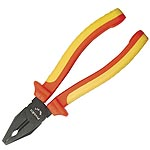
\includegraphics[width=\columnwidth]{fig/00/pros/PM-911.jpg}
\textbf{PM-911 Пассатижи 1\,кВ}

\noindent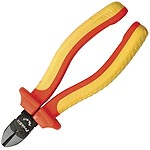
\includegraphics[width=\columnwidth]{fig/00/pros/PM-917.jpg}
\textbf{PM-917 Кусачки (бокорезы) 1\,кВ}

\subsubsection{Хранение}

\noindent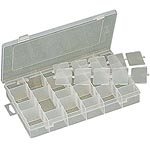
\includegraphics[width=\columnwidth]{fig/00/pros/103-132D.jpg}
\textbf{103-132D Кассетница для деталей и компонентов}

\noindent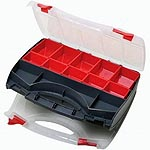
\includegraphics[width=\columnwidth]{fig/00/pros/SB-3428SB.jpg}
\textbf{SB-3428SB Портативная кассетница для саморезов и т.п.}

\subsubsection{Радиомонтаж}

\noindent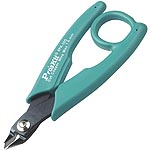
\includegraphics[width=\columnwidth]{fig/00/pros/8PK-30D.jpg}
\textbf{8PK-30D Кусачки миниатюрные}

\noindent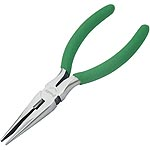
\includegraphics[width=\columnwidth]{fig/00/pros/1PK-709.jpg}
\textbf{1PK-709 Длинногубцы-кусачки}

\noindent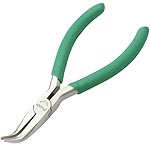
\includegraphics[width=\columnwidth]{fig/00/pros/1PK-055S.jpg}
\textbf{1PK-055S Длинногубцы изогнутые}

\noindent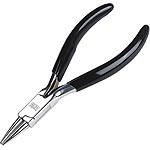
\includegraphics[width=\columnwidth]{fig/00/pros/1PK-29.jpg}
\textbf{1PK-29 Круглогубцы}

\noindent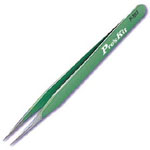
\includegraphics[width=\columnwidth]{fig/00/pros/1PK-101T.jpg}
\textbf{1PK-101T Пинцет прямой}

\noindent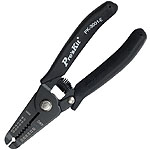
\includegraphics[width=\columnwidth]{fig/00/pros/1PK-3001E.jpg}
\textbf{1PK-3001E Клещи для зачистки проводов прецизионные (стриппер)}

\noindent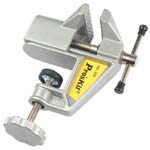
\includegraphics[width=\columnwidth]{fig/00/pros/PD-374.jpg}
\textbf{PD-374 Тиски на струбцине}

\subsubsection{Наборы}

\noindent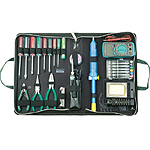
\includegraphics[width=\columnwidth]{fig/00/pros/1PK-616B.jpg}
\textbf{1PK-616B Набор инструментов для электроники профессиональный}

\noindent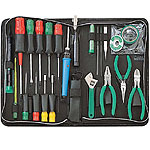
\includegraphics[width=\columnwidth]{fig/00/pros/1PK-813B.jpg}
\textbf{1PK-813B Набор базовых инструментов для электроники}

По личному опыту: в 1PK-813B не хватает мелкого мультиметра, стриппера
1PK-3001E, микрокусачек типа 8PK-30D, канифоли, ножа, настроечную 
отвертку заменить
индикаторной.

\end{multicols}



% \section{}
% \begin{multicols}{2}
% \end{multicols}

\end{document}